\documentclass[12pt, oneside]{article}
\usepackage[letterpaper, margin=1in, headsep=0.5in]{geometry}
\usepackage[english]{babel}
\usepackage[utf8]{inputenc}
\usepackage{amsmath}
\usepackage{amsfonts}
\usepackage{amssymb}
\usepackage{tikz}
\usetikzlibrary{quotes, angles}
\usepackage{graphicx}
%\usepackage{pgfplots}
%\pgfplotsset{width=10cm,compat=1.9}
%\usepgfplotslibrary{statistics}
%\usepackage{pgfplotstable}
%\usepackage{tkz-fct}
%\usepackage{venndiagram}

\usepackage{fancyhdr}
\pagestyle{fancy}
\fancyhf{}
\rhead{\thepage \\Name: \hspace{1.5in}.\\}
\lhead{BECA / Dr. Huson / Geometry 10th Grade\\* Unit 2: Introduction to Proof\\24 October 2018}

\renewcommand{\headrulewidth}{0pt}

\begin{document}
\subsubsection*{Pre-test problem set: Exam Friday}
  \vspace{0.5cm}
  \begin{enumerate}

  \item Complete the construction of an angle bisector including the six steps.
    \begin{enumerate}
      \item Given an angle with vertex $A$.
      \item Construct circle $A$ with arbitrary radius (i.e. the radius does not matter).
      \item Label the intersections $B$ and $C$ of the angle's rays and circle $A$.
      \item Construct circle $B$  with radius $BC$. \bigskip
      \item Construct circle $\rule{2cm}{0.15mm}$  with radius $\rule{2cm}{0.15mm}$. \bigskip
      \item Label $D$, the intersection of circle $B$ and $C$. \bigskip
      \item Draw ray $\rule{2cm}{0.15mm}$.
      \bigskip
      \item Ray $\overrightarrow {AD}$ bisects $\angle A$.
    \end{enumerate}
    \vspace{3cm}
    \begin{center}
    \begin{tikzpicture}
      \draw [<->, thick] (-2,6)--(0,0)--(9,0);
      \draw [fill] (0,0) circle [radius=0.05] node[below]{$A$};
      %\draw [fill] (7,0) circle [radius=0.05] node[below]{$N$};
    \end{tikzpicture}
    \end{center}
\newpage

  \item Construction a perpendicular to a line through a given point.\\
    Spicy: List the steps\\[0.5cm]
    \hspace{1cm} Given the line  $l$ and point $P$.
    \vspace{10cm}
    \begin{center}
    \begin{tikzpicture}
      \draw [<->, thick] (-2,0)--(9,0);
      \draw [fill] (2,3) circle [radius=0.05] node[right]{$P$};
      \node at (8.5,-0.4){$l$};
      %\draw [fill] (6,0) circle [radius=0.05] node[below]{$Q$};
    \end{tikzpicture}
    \end{center}
\newpage
  \item Points that are all located on the same plane are $\rule{4cm}{0.15mm}$. \bigskip

  \item Given the conditional statement, ``If a quadrilateral has congruent diagonals, then it is a rectangle."
    \begin{enumerate}
      \item Write down the hypothesis. \vspace{1.5cm}
      \item Write down the converse of the statement. \vspace{1.5cm}
      \item Write down the negation of the conclusion of the statement. \vspace{1.5cm}
    \end{enumerate}

  \item Given $A(2,4)$ and $B(6,9)$, find the coordinates of the midpoint of $\overline{AB}$, the point $M$.
    \vspace{5cm}

  \item Given $m \angle A=65$, $m \angle B=42$, $m \angle 1=50$, $m \angle DEF=132$, $m \angle FEG=48$. \bigskip
    \begin{enumerate}
      \item Find a pair of complementary angles. \rule{3cm}{0.15mm} \hspace{1cm} \rule{3cm}{0.15mm} \bigskip
      \item Find a pair of supplementary angles. \rule{3cm}{0.15mm} \hspace{1cm} \rule{3cm}{0.15mm} \bigskip
    \end{enumerate}

    \item Find the value of $|\pi-\frac{2}{5}|+\pi$. \vspace{2cm}

\newpage
  \item Given $R(-3,4)$ and $S(3,12)$, find the length of $\overline{RS}$.
      \vspace{4cm}

  \item In a proof, each of the following statements are written. Write down the reason that would justify each step. \bigskip
    \begin{enumerate}
      \item $\overline{BC} \cong \overline{BC}$ \hspace{4cm} $\rule{5cm}{0.15mm}$ property \bigskip
      \item $XY + BC= YZ+BC$  \hspace{1.7cm} $\rule{5cm}{0.15mm}$ property \bigskip
      \item $2(XY + YZ)=2XY+2YZ$  \hspace{0.8cm} $\rule{5cm}{0.15mm}$ property
    \end{enumerate} \bigskip

  \item Given $\overline{ABC}$, $AC=9$, and the point $B$ partitions $\overline{AC}$ in a ratio of 2:1.\\[0.5cm] Find ${AB}$. \\[0.5cm]
      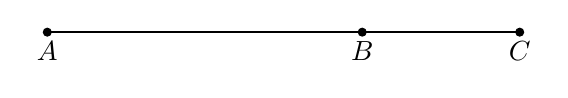
\begin{tikzpicture}
        \draw [-, thick] (1,0)--(7,0);
        \draw [fill] (1,0) circle [radius=0.05] node[below]{$A$};
        \draw [fill] (5,0) circle [radius=0.05] node[below]{$B$};
        \draw [fill] (7,0) circle [radius=0.05] node[below]{$C$};
      \end{tikzpicture} \vspace{3cm}

  \item Given rectangle $MATH$ with $MA=12.5$ and $AT=7.25$.
    \begin{enumerate}
      \item Find the perimeter of $MATH$. \vspace{2cm}
      \item Find the area of $MATH$.
    \end{enumerate}

\newpage
  \item Given the situation in the diagram, answer each question. Circle True or False. \vspace{1cm}
      \begin{flushright}
      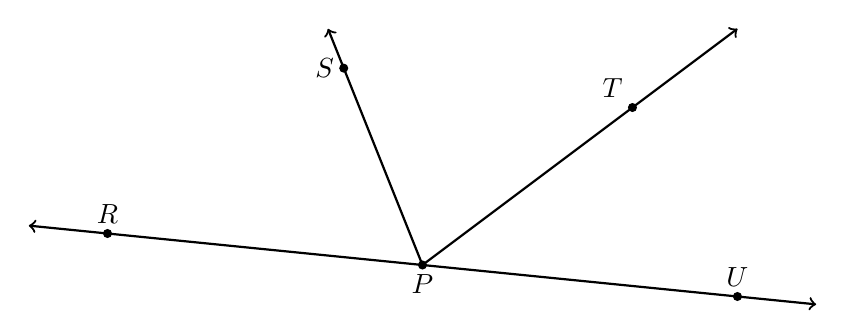
\begin{tikzpicture}[scale=1]
        \draw [->, thick] (0,0)--(4,3);
        \draw [<->, thick] (-5,.5)--(5,-.5);
        \draw [->, thick] (0,0)--(-1.2,3);
        \draw [fill] (-1,2.5) circle [radius=0.05] node[left ]{$S$};
        \draw [fill] (2.66666,2) circle [radius=0.05] node[above left ]{$T$};
        \draw [fill] (0,0) circle [radius=0.05] node[below]{$P$};
        \draw [fill] (4,-0.4) circle [radius=0.05] node[above]{$U$};
        \draw [fill] (-4,0.4) circle [radius=0.05] node[above]{$R$};
      \end{tikzpicture}
      \end{flushright}
    \begin{enumerate}
      \item True or False: $\overrightarrow{PR}$ and $\overrightarrow{PU}$ are opposite rays.\bigskip
      \item True or False: $\angle TPU$ is an acute angle.\bigskip
      \item True or False: $\angle RPT$ and $\angle TPU$ are complementary angles.\bigskip
      \item True or False: $\angle RPT$ and $\angle UPT$ are adjacent. \bigskip
    \end{enumerate}

  \item Given the circle $C$ with area $64\pi$. Find the circumference of $C$. \vspace{4cm}

  \item Find the length of a line segment with one end point of $(5,7)$ and a midpoint of $(10, -5)$. \vspace{5cm}

\newpage
  \item Given $m\angle RSU$ is three times $m\angle TSU$. Find $m\angle TSU$.\\[1cm]
    \begin{tikzpicture}[scale=2]
      %\draw [->, thick] (0,0)--(5,5);
      \draw [<-, thick] (-1,0)--(3,0)--(2,1.5)--(1,0);
      \draw [fill] (-0.5,0) circle [radius=0.025] node[below]{$R$};
      \draw [fill] (1,0) circle [radius=0.025] node[below]{$S$};
      \draw [fill] (2,1.5) circle [radius=0.025] node[right]{$U$};
      \draw [fill] (3,0) circle [radius=0.025] node[right]{$T$};
    \end{tikzpicture}
\vspace{3cm}

  \item Given $\overleftrightarrow{QS}$ as shown on the number line, with $Q$ having the coordinate 2.15 and $S$ the coordinate 5.63. \\[20pt] % Midpoint
    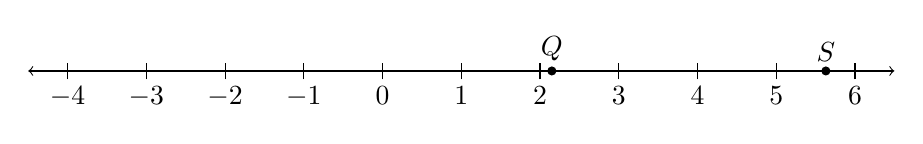
\begin{tikzpicture}
      \draw [<->] (-4.5,0)--(6.5,0);
      \foreach \x in {-4,...,6} %2 leading for diff!=1
        \draw[shift={(\x,0)},color=black] (0pt,-3pt) -- (0pt,3pt) node[below=5pt]  {$\x$};
        \draw [fill] (2.15,0) circle [radius=0.05] node[above] {$Q$};
        \draw [fill] (5.63,0) circle [radius=0.05] node[above] {$S$};
    \end{tikzpicture} \bigskip
    \begin{enumerate}
      \item Find the value of the coordinate of the point $R$, the midpoint of $\overline{QS}$. \vspace{4cm}
      \item The point $P$ is collinear with $\overleftrightarrow{QS}$ such that $Q$ is the midpoint of $\overleftrightarrow{PS}$. Mark $P$ on the line and state the value of its coordinate.
    \end{enumerate}\vspace{4cm}


\newpage
    \item Given two vertical angles, $m \angle 1 = \frac{5}{6}(5x-13)$, $m \angle 2 = \frac{5}{6}(4x+4)$. Find $m \angle 1$.
    \begin{enumerate}
      \item First label the drawing.
      \begin{flushright}
      \begin{tikzpicture}[scale=.7]
        \draw [<->, thick] (0,-1.5)--(10,1.5);
        \draw [<->, thick] (2,3.5)--(7,-3.5);
        \node at (3,.4){1};
        \node at (6,-.6){2};
        %\draw [fill] (0,0) circle [radius=0.05] node[below]{$P$};
        %\draw [fill] (6,0) circle [radius=0.05] node[below]{$R$};
        %\draw [fill] (3,0) circle [radius=0.05] node[below]{$Q$};
      \end{tikzpicture}
      \end{flushright}
      \vspace{1cm}
      \item Write a geometric equation: \rule{4cm}{0.15mm} \hspace{1cm} \rule{4cm}{0.15mm}
      \begin{flushright} State the reason \end{flushright}
      \vspace{.7cm}
      \item Substitute algebraic values: \rule{4cm}{0.15mm}
      \item Solve for $x$
      \vspace{4cm}
      %\begin{center} $x=$ \rule{1cm}{0.15mm} \end{center}
      \item Answer the question:
      \vspace{3cm}
      \item Check your answer
    \end{enumerate}

\newpage
  \item Given $\overrightarrow{BA} \perp \overrightarrow{BC}$, $m \angle ABD = 8x+1$, and $m \angle DBC = 4x-7$. Find $m \angle DBC$.\\[0.5cm]
    First label the drawing.
    \begin{flushright}
    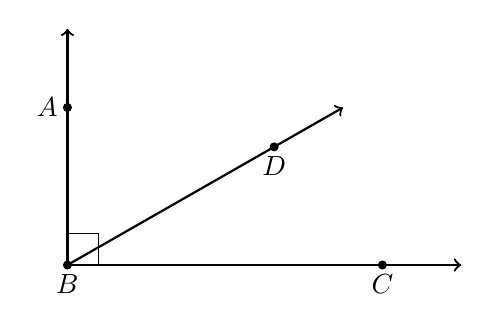
\begin{tikzpicture}[scale=1]
      \draw [<->, thick] (0,3)--(0,0)--(5,0);
      \draw [->, thick] (0,0)--(3.5, 2);
      \draw [-, thin] (0, 0.4)--(0.4, 0.4)--(0.4, 0);
      %\node at (3,.4){1};
      %\node at (6,-.6){2};
      \draw [fill] (0,0) circle [radius=0.05] node[below]{$B$};
      \draw [fill] (0,2) circle [radius=0.05] node[left]{$A$};
      \draw [fill] (4,0) circle [radius=0.05] node[below]{$C$};
      \draw [fill] (2.625, 1.5) circle [radius=0.05] node[below]{$D$};
    \end{tikzpicture}
    \end{flushright}
    %\vspace{.5cm}
    \begin{enumerate}
      \item Write a geometric equation: \rule{4cm}{0.15mm} \hspace{1cm} \rule{4cm}{0.15mm}
      \vspace{.5cm}
      \item Substitute algebraic values: \rule{4cm}{0.15mm} \bigskip
      \item Solve for $x$
      \vspace{2cm}
      %\begin{center} $x=$ \rule{1cm}{0.15mm} \end{center}
      \item Answer the question:
      \vspace{2cm}
      \item Check your answer
    \end{enumerate}

  \end{enumerate}

\end{document}
